\chapter{Sorting}

\section{Introduction}
Why sortin is important

Give an example of sortin
\begin{description}
\item[Stable] When sorting some kinds of data, only part of the data is examined when determining the sort order. For example a deck of card can be orderd by means of the rank ignoring the seed yelding to multiple different valid sorting. A stable sorting algorithm ensure that the order of equal element will be preserved. 
\item[Adaptive]	A sorting algorithm falls into the adaptive sort family if it takes advantage of existing order in its input.  It benefits from the presortedness in the input sequence (or limited disorder) to sort faster. Time complexity is function of input size and entropy.
\item [Online] Online; i.e., can sort a list as it receives it
\end{description}

\section{Bubble-Sort}
Bubble sort, sometimes referred to as sinking sort, is a simple sorting algorithm that repeatedly steps through the list to be sorted, compares each pair of adjacent items and swaps them if they are in the wrong order. The pass through the list is repeated until no swaps are needed, which indicates that the list is sorted. The algorithm, which is a comparison sort, is named for the way smaller elements "bubble" to the top of the list. Although the algorithm is simple, it is too slow and impractical for most problems even when compared to insertion sort (see \ref{sec:insertionsort} at page \pageref{sec:insertionsort}). \textbf{Bubble sort is stable and adaptive}.

The distance and direction that elements must move during the sort determine bubble sort's performance because elements move in different directions at different speeds. An element that must move toward the end of the list can move quickly because it can take part in successive swaps. For example, the largest element in the list will win every swap, so it moves to its sorted position on the first pass even if it starts near the beginning. On the other hand, an element that must move toward the beginning of the list cannot move faster than one step per pass, so elements move toward the beginning very slowly. If the smallest element is at the end of the list, it will take $n-1$ passes to move it to the beginning. This has led to these types of elements being named rabbits and turtles, respectively, after the characters in Aesop's fable of The Tortoise and the Hare.

\begin{lstlisting}[language=C++, caption="Bubble-sort implementation in C++14"]
// CMP_FN has type: D -> D -> bool
template <typename Iterator, typename CMP_FN>
void bubblesort(Iterator s, Iterator e, CMP_FN cmp) {
  auto it1 = s;
  for (; it1 != e; it1++) {
    auto it2 = s;
    for (; it2 != it1; it2++)
      if (cmp(*it1, *it2)) 
      		std::swap(*it1, *it2);
  }
}
\end{lstlisting}

\subsection{Complexity Analysis}
Complexity is $\mathcal{O}(n^2)$ in worst and averge case. Being adaptive it takes advantage of already sorted (or nearly sorted) input. In this case the complexity is $\mathcal{O}(2n)$.
Bubble sort is asymptotically equivalent in running time to insertion sort in the worst case, but the two algorithms differ greatly in the number of swaps necessary. Experimental results such as those of Astrachan have also shown that insertion sort performs considerably better even on random lists. For these reasons many modern algorithm textbooks avoid using the bubble sort algorithm in favor of insertion sort.
Bubble sort also interacts poorly with modern CPU hardware. It requires at least twice as many writes as insertion sort, twice as many cache misses, and asymptotically more branch mispredictions. Experiments by Astrachan sorting strings in Java show bubble sort to be roughly one-fifth as fast as an insertion sort and $70\%$ as fast as a selection sort.
The only significant advantage that bubble sort has over most other implementations, even quicksort, but not insertion sort, is that the ability to detect that the list is sorted efficiently is built into the algorithm. When the list is already sorted (best-case), the complexity of bubble sort is only $\mathcal{O}(2n)$

\section{Insertion-Sort}
\label{sec:insertionsort}
Insertion sort is a simple sorting algorithm that builds the final sorted array (or list) one item at a time. It is much less efficient on large lists than more advanced algorithms such as quicksort, heapsort, or merge sort. However, insertion sort provides several advantages.
It is more efficient in practice than most other simple quadratic (i.e., $\mathcal{O}(n^2)$) algorithms such as selection sort or bubble sort. It is stable and adaptive.Infact when the input is nearly sorted its complexity becomes $\mathcal{O}(nk)$ (when each element is no more than k places away from its sorted position). Can also be easily implemented in-place (using $\mathcal{O}(1)$ additional memory).

It works keeping the first part of the data sorted and iterating on the rest of the data. For each element not already sorted the method finds its sorted position in the first part (the already sorted) of the data.

Sorting is typically done in-place, by iterating up the array, growing the sorted list behind it. At each array-position, it checks the value there against the largest value in the sorted list (which happens to be next to it, in the previous array-position checked). If larger, it leaves the element in place and moves to the next. If smaller, it finds the correct position within the sorted list, shifts all the larger values up to make a space, and inserts into that correct position.
The resulting array after k iterations has the property where the first k + 1 entries are sorted ("+1" because the first entry is skipped). In each iteration the first remaining entry of the input is removed, and inserted into the result at the correct position, thus extending the result:

\begin{figure}
		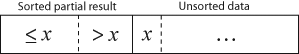
\includegraphics[width=8cm]{Insertionsort-before.png}
\end{figure}

\begin{figure}
		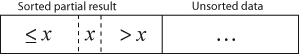
\includegraphics[width=8cm]{Insertionsort-after.png}
	\end{figure}


\begin{lstlisting}[language=c++, caption="Bubble-sort implementation in C++14"]
// CMP_FN has type: D -> D -> bool
template < typename Container, typename CMP_FN>
void insertionsort(Container& v, const int s,const int e, CMP_FN cmp) {
    for(int i=s+1 ; i<e; i++){
        int el = v[i];
        int j = i-1;
        while(cmp(el,v[j]) && j>=s){
            v[j+1] = v[j];
            j--;
        }
        v[j+1]=el;
    }
}
\end{lstlisting}

Suppose we have an array A, and that the subarray from index 0 through index $k$ is already sorted, and we want to insert the element currently in index $k+1$ into this sorted subarray, so that the subarray from index 0 through index $k+1$ is sorted. 
To insert the element in position $k+1$ into the subarray to its left, we repeatedly compare it with elements to its left , going right to left. Let's call the element in position $k+1$ the key. Each time we find that the key is less than an element to its left, we slide that element one position to the right, since we know that the key will have to go to that element's left. We'll need to do two things to make this idea work: we need to have a slide operation that slides an element one position to the right, and we need to save the value of the key in a separate place (so that it doesn't get overridden by the element to its immediate left). 

Here an Haskell implementation of \textit{insertion sort}
\begin{lstlisting}[language=Haskell,caption="Haskell Insertion sort "]
 insert :: Ord a => a -> [a] -> [a]
 insert item []  = [item]
 insert item (h:t) | item <= h = item:h:t
                   | otherwise = h:(insert item t)

 insertsort :: Ord a => [a] -> [a]
 insertsort []    = []   
 insertsort (h:t) = insert h (insertsort t)
\end{lstlisting}

\subsection{Complexity Analysis}
Time complexity is  $\mathcal{O}(n^2)$ while spatial complexity is  $\mathcal{O}(1)$. It is adaptive, and when each element does not move more than $k$ position from the original position to the sorted location its complexity is linear:  $\mathcal{O}(nk)$.   As for bubble-sort its best case is linear, but it performs much less operations mainly because bubble-sort is a \textit{exchange} algorithm while insertion sort is a \textit{shifting} one. Exchange requires a third of the operation of \textit{shifting}.

\section{Selection-Sort}
Selection sorting is conceptually the most simplest sorting algorithm. This algorithm first finds the smallest element in the array and exchanges it with the element in the first position, then find the second smallest element and exchange it with the element in the second position, and continues in this way until the entire array is sorted. 

The algorithm divides the input list into two parts: the sublist of items already sorted, which is built up from left to right at the front (left) of the list, and the sublist of items remaining to be sorted that occupy the rest of the list. Initially, the sorted sublist is empty and the unsorted sublist is the entire input list. The algorithm proceeds by finding the smallest (or largest, depending on sorting order) element in the unsorted sublist, exchanging (swapping) it with the leftmost unsorted element (putting it in sorted order), and moving the sublist boundaries one element to the right.

\begin{verbatim}
64 25 12 22 11 // this is the initial, starting state of the array

11 25 12 22 64 // sorted sublist = {11}

11 12 25 22 64 // sorted sublist = {11, 12}

11 12 22 25 64 // sorted sublist = {11, 12, 22}

11 12 22 25 64 // sorted sublist = {11, 12, 22, 25}

11 12 22 25 64 // sorted sublist = {11, 12, 22, 25, 64}
\end{verbatim}
\subsection{Complexity Analysis}
Time complexity is  $\mathcal{O}(n^2)$ and is generally slower than insertion sort and is not used in production code except when memory is very limited.





\section{Merge-Sort}
In computer science, merge sort (also commonly spelled mergesort) is an efficient, general-purpose, comparison-based sorting algorithm. Most implementations produce a stable sort, which means that the implementation preserves the input order of equal elements in the sorted output. Mergesort is a divide and conquer algorithm that was invented by John von Neumann in 1945.

Conceptually, a merge sort works as follows:
\begin{enumerate}
\item Divide the unsorted list into n sublists, each containing 1 element (a list of 1 element is considered sorted).
\item Repeatedly merge sublists to produce new sorted sublists until there is only 1 sublist remaining. This will be the sorted list.
\end{enumerate} 

Merge is the most important part of the algorithm. Merge algorithms are a family of algorithms that take multiple sorted lists as input and produce a single list as output, containing all the elements of the inputs lists in sorted order. These algorithms are used as subroutines in various sorting algorithms, most famously merge sort.

In particular merging two sorted collections into one can be done in linear time and linear space.When the inputs are linked lists, this algorithm can be implemented to use only a constant amount of working space; the pointers in the lists' nodes can be reused for bookkeeping and for constructing the final merged list.

\begin{lstlisting}[language=c++, caption="Bubble-sort implementation in C++14"]
// CMP_FN has type: D -> D -> bool
//[s1,e1] and [e1+1,e2] are two ordered sequences. This methods reaggarne the whole
// interval [s1,e2] in a sorted sequence
template < typename Container, typename CMP_FN>
void merge(Container& v, Container& scratch,  int s1,  int e1,  int e2,CMP_FN cmp){
    int s2 = e1+1;
    int ins =0;
    int b = s1;
    while(s1 <= e1 && s2<=e2)
        if(cmp(v[s1],v[s2]))
            scratch[b+ins++] = v[s1++];
        else
            scratch[b+ins++] = v[s2++];
    while(s1 <= e1)
        scratch[b+ins++] = v[s1++];
    while(s2 <= e2)
        scratch[b+ins++] = v[s2++];
        
    for(int i=0 ; i < ins ; i++)
        v[b+i] = scratch[b+i];
}
\end{lstlisting}


In the merge sort algorithm, this subroutine is typically used to merge two sub-arrays $A[lo..mid]$, $A[mid..hi]$ of a single array $A$. This can be done by copying the sub-arrays into a temporary array, then applying the merge algorithm above.The allocation of a temporary array can be avoided, but at the expense of speed and programming ease. Various in-place merge algorithms have been devised, sometimes sacrificing the linear-time bound to produce an $\mathcal{nlog(n)}(n^2)$ algorithm.

\subsection{Complexity Analysis}

\section{Quick-Sort}

\subsection{Complexity Analysis}

\section{Heap-Sort}

\subsection{Complexity Analysis}

\section{Smoot-Sort}

\subsection{Complexity Analysis}